\documentclass{standalone}
\usepackage{tikz}
\usetikzlibrary{patterns, positioning}


\begin{document}
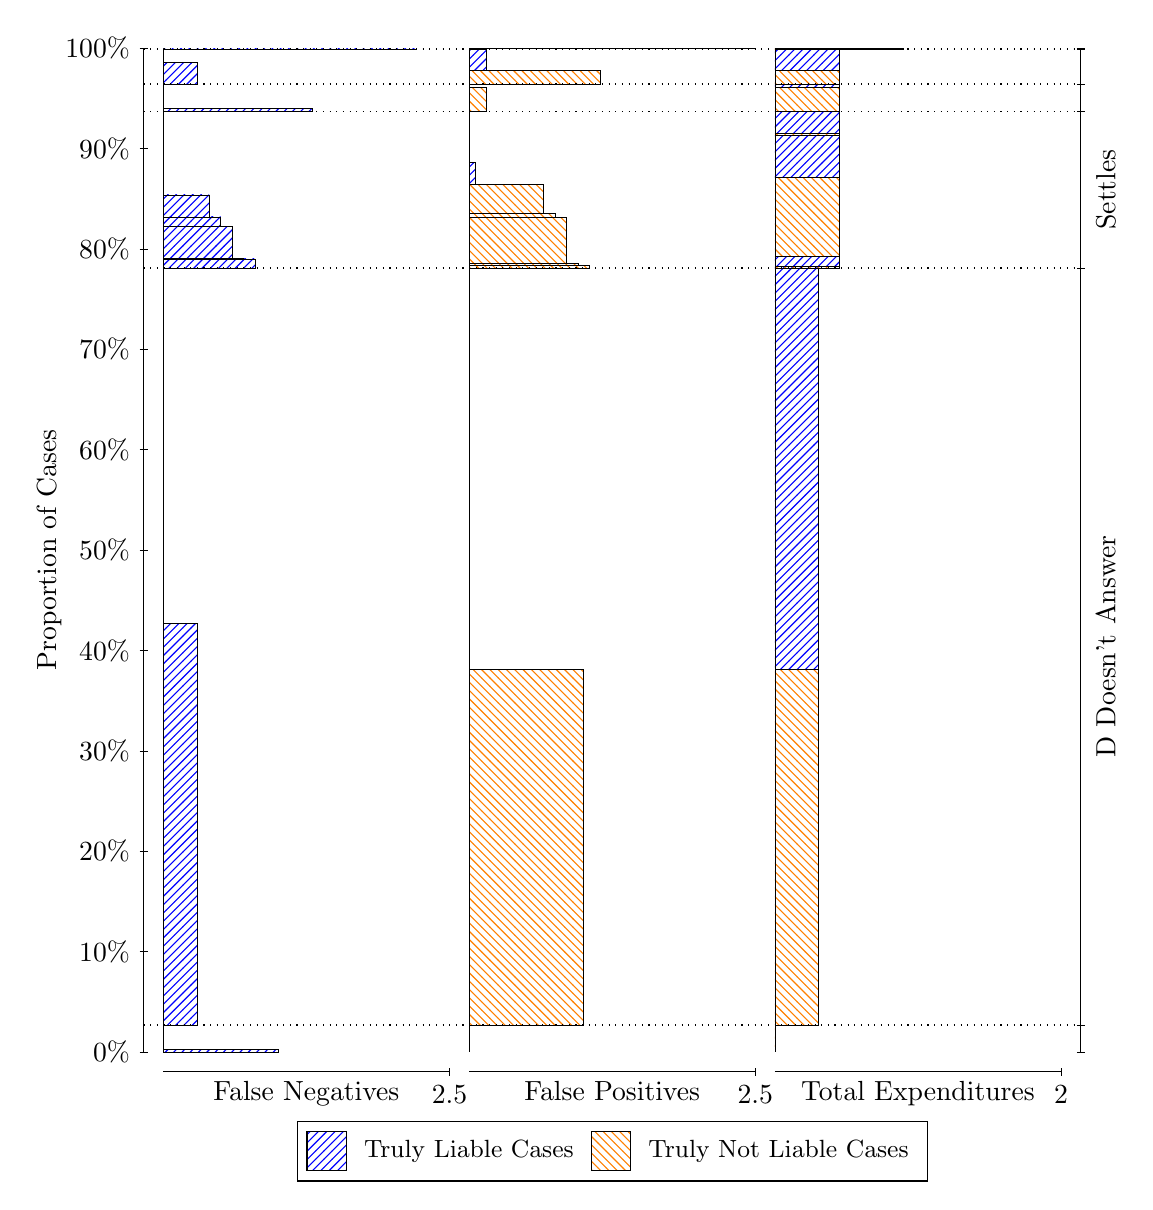
\begin{tikzpicture}
\draw[black, very thin] (1.5,1.75) -- (1.5,14.5);
\node[rotate=90, text=black, anchor=center] at (0.3, 8.125) {Proportion of Cases};
\draw[black, very thin] (1.45,1.75) -- (1.55,1.75);
\node[text=black, anchor=east] at (1.45, 1.75) {0\%};
\draw[black, very thin] (1.45,3.025) -- (1.55,3.025);
\node[text=black, anchor=east] at (1.45, 3.025) {10\%};
\draw[black, very thin] (1.45,4.3) -- (1.55,4.3);
\node[text=black, anchor=east] at (1.45, 4.3) {20\%};
\draw[black, very thin] (1.45,5.575) -- (1.55,5.575);
\node[text=black, anchor=east] at (1.45, 5.575) {30\%};
\draw[black, very thin] (1.45,6.85) -- (1.55,6.85);
\node[text=black, anchor=east] at (1.45, 6.85) {40\%};
\draw[black, very thin] (1.45,8.125) -- (1.55,8.125);
\node[text=black, anchor=east] at (1.45, 8.125) {50\%};
\draw[black, very thin] (1.45,9.4) -- (1.55,9.4);
\node[text=black, anchor=east] at (1.45, 9.4) {60\%};
\draw[black, very thin] (1.45,10.675) -- (1.55,10.675);
\node[text=black, anchor=east] at (1.45, 10.675) {70\%};
\draw[black, very thin] (1.45,11.95) -- (1.55,11.95);
\node[text=black, anchor=east] at (1.45, 11.95) {80\%};
\draw[black, very thin] (1.45,13.225) -- (1.55,13.225);
\node[text=black, anchor=east] at (1.45, 13.225) {90\%};
\draw[black, very thin] (1.45,14.5) -- (1.55,14.5);
\node[text=black, anchor=east] at (1.45, 14.5) {100\%};

\draw[black, very thin] (13.4,1.75) -- (13.4,14.5);
\draw[black, very thin] (13.35,1.75) -- (13.45,1.75);
\node[anchor=west] at (13.35, 1.75) {};
\draw[black, very thin] (13.35,2.092) -- (13.45,2.092);
\node[anchor=west] at (13.35, 2.092) {};
\draw[black, very thin] (13.35,11.707) -- (13.45,11.707);
\node[anchor=west] at (13.35, 11.707) {};
\draw[black, very thin] (13.35,13.698) -- (13.45,13.698);
\node[anchor=west] at (13.35, 13.698) {};
\draw[black, very thin] (13.35,14.043) -- (13.45,14.043);
\node[anchor=west] at (13.35, 14.043) {};
\draw[black, very thin] (13.35,14.486) -- (13.45,14.486);
\node[anchor=west] at (13.35, 14.486) {};
\draw[black, very thin] (13.35,14.495) -- (13.45,14.495);
\node[anchor=west] at (13.35, 14.495) {};
\draw[black, very thin] (13.35,14.5) -- (13.45,14.5);
\node[anchor=west] at (13.35, 14.5) {};

\draw[black, very thin, pattern color=blue, pattern=north east lines] (1.75,1.75) rectangle (3.2033,1.786);
\draw[black, very thin, pattern color=orange, pattern=north west lines] (1.75,1.786) rectangle (1.75,2.092);
\draw[black, very thin, pattern color=blue, pattern=north east lines] (1.75,2.092) rectangle (2.186,7.1887);
\draw[black, very thin, pattern color=orange, pattern=north west lines] (1.75,7.1887) rectangle (1.75,11.707);
\draw[black, very thin, pattern color=blue, pattern=north east lines] (1.75,11.707) rectangle (2.9127,11.823);
\draw[black, very thin, pattern color=blue, pattern=north east lines] (1.75,11.823) rectangle (2.7673,11.828);
\draw[black, very thin, pattern color=blue, pattern=north east lines] (1.75,11.828) rectangle (2.622,12.231);
\draw[black, very thin, pattern color=blue, pattern=north east lines] (1.75,12.231) rectangle (2.4767,12.356);
\draw[black, very thin, pattern color=blue, pattern=north east lines] (1.75,12.356) rectangle (2.3313,12.634);
\draw[black, very thin, pattern color=orange, pattern=north west lines] (1.75,12.634) rectangle (1.75,13.698);
\draw[black, very thin, pattern color=blue, pattern=north east lines] (1.75,13.698) rectangle (3.6393,13.736);
\draw[black, very thin, pattern color=orange, pattern=north west lines] (1.75,13.736) rectangle (1.75,14.043);
\draw[black, very thin, pattern color=blue, pattern=north east lines] (1.75,14.043) rectangle (2.186,14.316);
\draw[black, very thin, pattern color=orange, pattern=north west lines] (1.75,14.316) rectangle (1.75,14.486);
\draw[black, very thin, pattern color=blue, pattern=north east lines] (1.75,14.486) rectangle (4.9473,14.488);
\draw[black, very thin, pattern color=orange, pattern=north west lines] (1.75,14.488) rectangle (1.75,14.495);
\draw[black, very thin, pattern color=orange, pattern=north west lines] (1.75,14.495) rectangle (1.75,14.498);
\draw[black, very thin, pattern color=blue, pattern=north east lines] (1.75,14.498) rectangle (1.75,14.5);
\draw[black, very thin, pattern color=orange, pattern=north west lines] (5.6333,1.75) rectangle (5.6333,2.056);
\draw[black, very thin, pattern color=blue, pattern=north east lines] (5.6333,2.056) rectangle (5.6333,2.092);
\draw[black, very thin, pattern color=orange, pattern=north west lines] (5.6333,2.092) rectangle (7.0867,6.6105);
\draw[black, very thin, pattern color=blue, pattern=north east lines] (5.6333,6.6105) rectangle (5.6333,11.707);
\draw[black, very thin, pattern color=orange, pattern=north west lines] (5.6333,11.707) rectangle (7.1593,11.741);
\draw[black, very thin, pattern color=orange, pattern=north west lines] (5.6333,11.741) rectangle (7.014,11.761);
\draw[black, very thin, pattern color=orange, pattern=north west lines] (5.6333,11.761) rectangle (6.8687,12.345);
\draw[black, very thin, pattern color=orange, pattern=north west lines] (5.6333,12.345) rectangle (6.7233,12.397);
\draw[black, very thin, pattern color=orange, pattern=north west lines] (5.6333,12.397) rectangle (6.578,12.771);
\draw[black, very thin, pattern color=blue, pattern=north east lines] (5.6333,12.771) rectangle (5.706,13.049);
\draw[black, very thin, pattern color=blue, pattern=north east lines] (5.6333,13.049) rectangle (5.6333,13.698);
\draw[black, very thin, pattern color=orange, pattern=north west lines] (5.6333,13.698) rectangle (5.8513,14.004);
\draw[black, very thin, pattern color=blue, pattern=north east lines] (5.6333,14.004) rectangle (5.6333,14.043);
\draw[black, very thin, pattern color=orange, pattern=north west lines] (5.6333,14.043) rectangle (7.3047,14.213);
\draw[black, very thin, pattern color=blue, pattern=north east lines] (5.6333,14.213) rectangle (5.8513,14.486);
\draw[black, very thin, pattern color=orange, pattern=north west lines] (5.6333,14.486) rectangle (5.6333,14.493);
\draw[black, very thin, pattern color=blue, pattern=north east lines] (5.6333,14.493) rectangle (5.6333,14.495);
\draw[black, very thin, pattern color=orange, pattern=north west lines] (5.6333,14.495) rectangle (9.2667,14.498);
\draw[black, very thin, pattern color=blue, pattern=north east lines] (5.6333,14.498) rectangle (7.8133,14.5);
\draw[black, very thin, pattern color=orange, pattern=north west lines] (9.5167,1.75) rectangle (9.5167,2.056);
\draw[black, very thin, pattern color=blue, pattern=north east lines] (9.5167,2.056) rectangle (9.5167,2.092);
\draw[black, very thin, pattern color=orange, pattern=north west lines] (9.5167,2.092) rectangle (10.062,6.6105);
\draw[black, very thin, pattern color=blue, pattern=north east lines] (9.5167,6.6105) rectangle (10.062,11.707);
\draw[black, very thin, pattern color=orange, pattern=north west lines] (9.5167,11.707) rectangle (10.334,11.727);
\draw[black, very thin, pattern color=blue, pattern=north east lines] (9.5167,11.727) rectangle (10.334,11.852);
\draw[black, very thin, pattern color=orange, pattern=north west lines] (9.5167,11.852) rectangle (10.334,12.862);
\draw[black, very thin, pattern color=blue, pattern=north east lines] (9.5167,12.862) rectangle (10.334,13.386);
\draw[black, very thin, pattern color=orange, pattern=north west lines] (9.5167,13.386) rectangle (10.334,13.42);
\draw[black, very thin, pattern color=blue, pattern=north east lines] (9.5167,13.42) rectangle (10.334,13.698);
\draw[black, very thin, pattern color=orange, pattern=north west lines] (9.5167,13.698) rectangle (10.334,14.004);
\draw[black, very thin, pattern color=blue, pattern=north east lines] (9.5167,14.004) rectangle (10.334,14.043);
\draw[black, very thin, pattern color=orange, pattern=north west lines] (9.5167,14.043) rectangle (10.334,14.213);
\draw[black, very thin, pattern color=blue, pattern=north east lines] (9.5167,14.213) rectangle (10.334,14.486);
\draw[black, very thin, pattern color=orange, pattern=north west lines] (9.5167,14.486) rectangle (11.152,14.493);
\draw[black, very thin, pattern color=blue, pattern=north east lines] (9.5167,14.493) rectangle (11.152,14.495);
\draw[black, very thin, pattern color=orange, pattern=north west lines] (9.5167,14.495) rectangle (11.152,14.498);
\draw[black, very thin, pattern color=blue, pattern=north east lines] (9.5167,14.498) rectangle (11.152,14.5);
\draw[black, dotted] (1.5,2.092) -- (13.4,2.092);
\draw[black, dotted] (1.5,11.707) -- (13.4,11.707);
\draw[black, dotted] (1.5,13.698) -- (13.4,13.698);
\draw[black, dotted] (1.5,14.043) -- (13.4,14.043);
\draw[black, dotted] (1.5,14.486) -- (13.4,14.486);
\draw[black, dotted] (1.5,14.495) -- (13.4,14.495);
\draw[black, very thin] (1.75,1.5) -- (5.3833,1.5);
\node[text=black, anchor=north] at (3.5667, 1.5) {False Negatives};
\draw[black, very thin] (5.3833,1.45) -- (5.3833,1.55);
\node[text=black, anchor=north] at (5.3833, 1.45) {2.5};

\draw[black, very thin] (5.6333,1.5) -- (9.2667,1.5);
\node[text=black, anchor=north] at (7.45, 1.5) {False Positives};
\draw[black, very thin] (9.2667,1.45) -- (9.2667,1.55);
\node[text=black, anchor=north] at (9.2667, 1.45) {2.5};

\draw[black, very thin] (9.5167,1.5) -- (13.15,1.5);
\node[text=black, anchor=north] at (11.333, 1.5) {Total Expenditures};
\draw[black, very thin] (13.15,1.45) -- (13.15,1.55);
\node[text=black, anchor=north] at (13.15, 1.45) {2};


\node[text=black, centered, rotate=90] at (13.72, 6.8996) {D Doesn't Answer};
\node[text=black, centered, rotate=90] at (13.72, 12.702) {Settles};





\draw (7.449999999999999,1.5) node[draw=none] (baseCoordinate) {};
\begin{scope}[align=center]
        \matrix[scale=0.5, draw=black, below=0.5cm of baseCoordinate, nodes={draw}, column sep=0.1cm]{
            \node[rectangle, draw, minimum width=0.5cm, minimum height=0.5cm, pattern color=blue, pattern=north east lines] {}; &
            \node[draw=none, font=\small, text=black] (B) {Truly Liable Cases}; &
            \node[rectangle, draw, minimum width=0.5cm, minimum height=0.5cm, pattern color=orange, pattern=north west lines] {}; &
            \node[draw=none, font=\small, text=black] (B) {Truly Not Liable Cases}; \\
            };
\end{scope}

\end{tikzpicture}
\end{document}